%!TEX root = ../main.tex
\chapter{Differential Equations}

\section{Uniqueness of initial value problem}
Recall
\begin{theorem}[Uniqueness of initial value problem]
\label{uniqueivp}
If \(\Phi\) is continuous and satisfies a Lipschitz condition in \(y\) on the set
\[ \mathcal{D} = \Set{(t, y)}{t_0 \leq t \leq T, y\in\R}, \]
then
\[ \dot{y} = \Phi(t, y), \quad  y(t_0) = y_0, \text{ where } t_0 \leq t \leq T \]
has a unique solution.
\end{theorem}
\begin{enumerate}
	\item Show \(\Phi\) satisfies a Lipschitz condition in \(y\) on \(\mathcal{A}\) with Lipschitz constant \(c\) if \(\mathcal{A}\) is convex and there exists a \(c > 0\) such that
	\[ \left|\partial_{y}\Phi(t,y)\right|\leq c, \quad \forall (t,y)\in\mathcal{A} \]
	\item Show for any constants \(t_0\) and \(T\), the set \(\mathcal{D}\) is convex.
	\item Use the above to show the following IVP has a unique solution.
	\[ \dot{y}=\frac{4t^3y}{1+t^4}, \quad y(0)=1, \quad t\in[0,1]. \]
	\begin{proof}
	\[ |\Phi(t,y_1)-\Phi(t,y_2)|=\frac{4|t|^3}{1+t^4}\cdot|y_1-y_2|. \]
	So we can find a Lipschitz constant \(L\) as
	\[ L\geq \sup_{t\in[0,1]} \frac{4t^3}{1+t^4}=2. \]
	So we proved that \(\Phi(t,y)\) is Lipschitz continuous in \(y\).
	According to the \hyperref[uniqueivp]{uniqueness of initial value problem}, this IVP has a unique solution.
	\end{proof}
	\item Do you think it is a good idea to solve the following IVP numerically?
	\[ \dot{y}=1+y^2, \quad y(0)=0, \quad t\in[0,3]. \]
	Justify your answer.
	Show Euler's method is going to fail miserably for this IVP.
	\begin{proof}[Answer]
	No. The function \(\Phi(y)=1+y^2\) is not Lipschitz continuous on \(\R\), so Euler's method will fail.
	In practice, if we choose \(h=1\), then \(\hat{y}(3)=13\).
	If \(h=0.5\), then \(\hat{y}(3)=218.1344\).
	Table \ref{eulerdiverge} shows the estimation of \(y(3)\) from Euler's method with \(h\to0\).
	\ifnum\webview=1
		\begin{table}[H]
	\else
		\begin{table}[htbp]
	\fi
		\centering
		\begin{tabular}{|c|c|}
		\hline
		Steps & \(\hat{y}(3)\)	\\	\hline
		1	&	3	\\	\hline
		2	&	6.375000000000000	\\	\hline
		3	&	13	\\	\hline
		4	&	28.404234389774501	\\	\hline
		5	&	71.073212236802789	\\	\hline
		6	&	2.181344382569777e+02	\\	\hline
		7	&	8.937891513340965e+02	\\	\hline
		8	&	5.455818281020568e+03	\\	\hline
		9	&	5.729541345952547e+04	\\	\hline
		\end{tabular}
		\caption{Divergence of Euler's method on non-Lipschitz functions}
		\label{eulerdiverge}
	\end{table}
	Clearly, when \(h\to0\), \(\hat{y}(3)\) diverges quickly.
	\end{proof}
\end{enumerate}


\section{Initial value problem}
Consider the following IVP
\[ \dot{y} = \arctan(y), \quad y(0) = y_0, \quad t_0\leq t\leq T \]
\begin{enumerate}
	\item Find a Lipschitz constant for \(\arctan(y)\).
	\begin{proof}[Answer]
	Obviously,
	\[ L\leq\max_{y}\frac{\ud}{\ud y}\arctan(y)=\max_{y}\frac{1}{1+y^2}=1. \]
	So a Lipschitz constant can be \(L=1\).
	\end{proof}
	\item Find an upper bound on \(|\ddot{y}|\) without solving the IVP.
	\begin{proof}[Answer]
	Differentiate both sides of the equation,
	\[ \ddot{y}=\frac{1}{1+y^2}, \]
	so an upper bound is
	\[ \sup_{y\in\R}\frac{1}{1+y^2}=1. \]
	\end{proof}
	\item Find an upper bound on the absolute global error
	\[ |e_k|=|\hat{y}_k-y(t_k)|, \]
	where \(\hat{y}_k\) is the Euler's approximation to \(y(t_k)\), in terms of step size and \(t_k\).
	\begin{proof}[Answer]
	Since \(\Phi(y)=\arctan(y)\in\mathcal{C}^2(\R)\), we have
	\[ |e_k|\leq h\cdot\frac{\sup_{t}|\ddot{y}|}{2c}\left[e^{c(T-t_0)}-1 \right]. \]
	According to the previous result, the second derivative is bounded by 1, and the Lipschitz constant is also \(c=1\).
	Thus, the global error is bounded by
	\[ |e_k|\leq \frac{h}{2}\left[e^{T-t_0}-1 \right]. \]
	\end{proof}
\end{enumerate}


\section{Comparison of different methods}
Solve the following IVP using the step size \(h = 1\)
\[ \dot{y}=\left(2+0.01t^2\right)y, \quad y(0)=4, \quad t\in[0,15]. \]
\begin{enumerate}
	\item By Euler's method.
	\item By the backward Euler's method.
	\item By the second-order Taylor's method.
	\item By the Heun's method.
	\item By the two-step Adams-Bashforth method.
	\item It was mentioned in class that Heun's method, which is derived by applying the trapezoidal rule
	\[ \int_{a}^{b}f(x)\ud x\approx\frac{1}{2}(b-a)\left(f(a)+f(b)\right) \]
	is one the simplest form of Runge-Kutta method.
	The other simple second-order Runge-Kutta method, which is also known as the modified Euler's method, uses the mid-point rule
	\[ \int_{a}^{b}f(x)\ud x\approx(b-a)f\left(\frac{a+b}{2}\right). \]
	Use this information to derive this second-order Runge-Kutta method.
	Write a piece of pseudocode for it, then implement it to solve the above IVP.
	\item The most widely used Runge-Kutta method is a fourth-order Runge-Kutta method, which uses four sequential evaluations of \(\Phi\) during each time step, \textit{i.e.}, it has four stages.
	Similar to the previous two Runge-Kutta, it can be understood from a quadrature rule.
	In this case, Simpson's rule:
	\[ \int_{a}^{b}f(x)\ud x\approx\frac{b-a}{6}f\left[f(a)+4f\left(\frac{a+b}{2}\right)+f(b)\right]. \]
	This scheme proceeds as follows:
	\begin{align*}
	\hat{y}_0&=y_0\\
	\hat{y}_n&=\hat{y}_{n-1}+\frac{h}{6}(k_1+2k_2+2k_3+k_4)\\
	\text{where} \quad \Phi_1&=\Phi(t_{k-1},\hat{y}_{k-1})\\
	\Phi_2&=\Phi\left(t_{k-1}+\frac{h}{2},\hat{y}_{k-1}+\frac{h}{2}\Phi_1\right)\\
	\Phi_3&=\Phi\left(t_{k-1}+\frac{h}{2},\hat{y}_{k-1}+\frac{h}{2}\Phi_2\right)\\
	\Phi_4&=\Phi\left(t_{k-1}+h,\hat{y}_{k-1}+h\Phi_3\right)\\
	\end{align*}
	Use this fourth-order Runge-Kutta method to solve the above IVP.
	\item Compare all of the above approximations to the exact solution by plotting them on the same graph.
	\item Use the approximation from Euler's method to find the value of \(y\) at \(t=9.625\) by interpolation in Newton's form.
\end{enumerate}
\begin{proof}[Answer]
The table of \(y\) values solved by Euler's method, backward Euler's method, second-order Taylor's method, Heun's method, two-step Adams-Bashforth method are second-order Runge-Kutta method based on mid-point rule are listed in Table \ref{odecomparisontab}.
And the result from 4\(\text{th}\) order Runge-Kutta method is in Table \ref{rungekutta4}.
All the solutions are plotted in Figure \ref{odecomparisonfig}.
Since this function increases too fast, the normal plot cannot present much inforamtion.
Thus, it is in log scale.
Even in log scale, the function increases cubically, since the exact solution is
\[ y(t)=4 e^{\frac{t^3}{300}+2 t} \]


\ifnum\webview=1
	\begin{table}[H]
\else
	\begin{table}[htbp]
\fi
	\centering
	\begin{subtable}[t]{0.32\textwidth}
		\centering
		\begin{tabular}[t]{|c|c|}
		\hline
		\(t\)	&	\(\hat{y}(t)\)	\\	\hline
		0	&	4					\\	\hline
		1	&	12					\\	\hline
		2	&	36.1200000000000	\\	\hline
		3	&	109.804800000000	\\	\hline
		4	&	339.296832000000	\\	\hline
		5	&	1072.17798912000	\\	\hline
		6	&	3484.57846464000	\\	\hline
		7	&	11708.1836411904	\\	\hline
		8	&	40861.5609077545	\\	\hline
		9	&	148736.081704226	\\	\hline
		10	&	566684.471293103	\\	\hline
		11	&	2266737.88517241	\\	\hline
		12	&	9542966.49657585	\\	\hline
		13	&	42370771.2447968	\\	\hline
		14	&	198718917.138097	\\	\hline
		15	&	985645829.004960	\\	\hline
		\end{tabular}
		\caption{Euler's method}
	\end{subtable}
	\begin{subtable}[t]{0.32\textwidth}
		\centering
		\begin{tabular}[t]{|c|c|}
		\hline
		\(t\)	&	\(\hat{y}(t)\)	\\	\hline
		0	&	4					\\	\hline
		1	&	-3.960396039603961	\\	\hline
		2	&	3.808073115003809	\\	\hline
		3	&	-3.493645059636522	\\	\hline
		4	&	3.011762982445278	\\	\hline
		5	&	-2.409410385956222	\\	\hline
		6	&	1.771625283791340	\\	\hline
		7	&	-1.189010257578080	\\	\hline
		8	&	0.725006254620781	\\	\hline
		9	&	-0.400555941779437	\\	\hline
		10	&	0.200277970889718	\\	\hline
		11	&	-0.090623516239692	\\	\hline
		12	&	0.037140785344136	\\	\hline
		13	&	-0.013806983399307	\\	\hline
		14	&	0.004664521418685	\\	\hline
		15	&	-0.001435237359595	\\	\hline
		\end{tabular}
		\caption{Backward Euler's method}
	\end{subtable}
	\begin{subtable}[t]{0.32\textwidth}
		\centering
		\begin{tabular}[t]{|c|c|}
		\hline
		\(t\)	&	\(\hat{y}(t)\)	\\	\hline
		0	&	4					\\	\hline
		1	&	20					\\	\hline
		2	&	100.801000000000	\\	\hline
		3	&	518.197780800000	\\	\hline
		4	&	2748.54693925224	\\	\hline
		5	&	15207.1605054948	\\	\hline
		6	&	88676.7546976665	\\	\hline
		7	&	550221.527548081	\\	\hline
		8	&	3664502.88454660	\\	\hline
		9	&	26402010.3825813	\\	\hline
		10	&	207204297.583017	\\	\hline
		11	&	1781956959.21395	\\	\hline
		12	&	16878785415.5225	\\	\hline
		13	&	176835659041.346	\\	\hline
		14	&	2056253885115.72	\\	\hline
		15	&	26609570276505.6	\\	\hline
		\end{tabular}
		\caption{2\(^\text{nd}\) order Taylor's method}
	\end{subtable}
	\begin{subtable}[t]{0.32\textwidth}
		\centering
		\begin{tabular}[t]{|c|c|}
		\hline
		\(t\)	&	\(\hat{y}(t)\)	\\	\hline
		0	&	4					\\	\hline
		1	&	20.0600000000000	\\	\hline
		2	&	101.808512000000	\\	\hline
		3	&	529.078475161600	\\	\hline
		4	&	2847.60616901476	\\	\hline
		5	&	16046.2607623982	\\	\hline
		6	&	95635.7141438932	\\	\hline
		7	&	608549.176240422	\\	\hline
		8	&	4169657.24576412	\\	\hline
		9	&	30998065.8964596	\\	\hline
		10	&	251704295.079252	\\	\hline
		11	&	2245202312.10693	\\	\hline
		12	&	22106711005.4672	\\	\hline
		13	&	241224009149.457	\\	\hline
		14	&	2926336699793.90	\\	\hline
		15	&	39564072181213.5	\\	\hline
		\end{tabular}
		\caption{Heun's method}
	\end{subtable}
	\begin{subtable}[t]{0.32\textwidth}
		\centering
		\begin{tabular}[t]{|c|c|}
		\hline
		\(t\)	&	\(\hat{y}(t)\)	\\	\hline
		0	&	4					\\	\hline
		1	&	20.0200000000000	\\	\hline
		2	&	76.3803000000000	\\	\hline
		3	&	289.983918000000	\\	\hline
		4	&	1121.17559493000	\\	\hline
		5	&	4450.75132819320	\\	\hline
		6	&	18261.1674183208	\\	\hline
		7	&	77898.6048349593	\\	\hline
		8	&	347301.716339914	\\	\hline
		9	&	1625632.75002645	\\	\hline
		10	&	8019236.52581924	\\	\hline
		11	&	41821786.8782187	\\	\hline
		12	&	231164835.908113	\\	\hline
		13	&	1356851421.25443	\\	\hline
		14	&	8469420520.13577	\\	\hline
		15	&	56274387537.5278	\\	\hline
		\end{tabular}
		\caption{Adams-Bashforth method}
	\end{subtable}
	\begin{subtable}[t]{0.32\textwidth}
		\centering
		\begin{tabular}[t]{|c|c|}
		\hline
		\(t\)	&	\(\hat{y}(t)\)	\\	\hline
		0	&	4					\\	\hline
		1	&	20.0200000000000	\\	\hline
		2	&	101.203352250000	\\	\hline
		3	&	522.841818561562	\\	\hline
		4	&	2792.24326755076	\\	\hline
		5	&	15584.0681248543	\\	\hline
		6	&	91833.9914469929	\\	\hline
		7	&	576813.891978135	\\	\hline
		8	&	3895116.05992360	\\	\hline
		9	&	28497448.1176130	\\	\hline
		10	&	227424240.920712	\\	\hline
		11	&	1991383509.56199	\\	\hline
		12	&	19227031815.4658	\\	\hline
		13	&	205536970107.329	\\	\hline
		14	&	2440754089236.66	\\	\hline
		15	&	32280071169495.0	\\	\hline
		\end{tabular}
		\caption{2\(^\text{nd}\) order Runge-Kutta method based on mid-point rule}
	\end{subtable}

	\caption{Comparison of different methods to solve ODE}
	\label{odecomparisontab}
\end{table}


\ifnum\webview=1
	\begin{algorithm2e}[H]
\else
	\begin{algorithm2e}[htbp]
\fi
	\KwIn{function \(\Phi\), endpoints \(t_0,T\), initial condition \(y_0\), number of steps\(n\)}
	\KwOut{\(t\) contains \(n+1\) equally spaced mesh points, starting from \(t_0\) to \(T\).\\
	\(y\) contains \(y_0\) and approximations to the solution at the corresponding \(t\)}
	\SetKwFunction{KwFn}{Runge-Kutta-2\(^\text{nd}\)-order}
	\KwFn(\(\Phi,t_0,T,y_0\)){:\\ }
	{
		\(h=(T-t_0)/n\)\;
		\(t[0]=t_0\)\;
		\(y[0]=y_0\)\;
		\For{\(i=1:n\)}
		{
			\(y[i]=y[i-1]+h\cdot\Phi\left(t[i-1]+h/2,y[i-1]+h/2\cdot\Phi(t[i-1],y[i-1])\right)\)\;
		}
	}

	\Return{\((t,y)\)}
	\caption{2\(^\text{nd}\) order Runge-Kutta method}
\end{algorithm2e}



\ifnum\webview=1
	\begin{table}[H]
\else
	\begin{table}[htbp]
\fi
		\centering
		\begin{tabular}[t]{|c|c|}
		\hline
		\(t\)	&	\(\hat{y}(t)\)	\\	\hline
		0	&	4					\\	\hline
		1	&	28.0867667083333	\\	\hline
		2	&	200.811414623582	\\	\hline
		3	&	1488.36689161515	\\	\hline
		4	&	11639.8029402688	\\	\hline
		5	&	97724.8224291606	\\	\hline
		6	&	895709.119604343	\\	\hline
		7	&	9107895.98380737	\\	\hline
		8	&	104325021.246580	\\	\hline
		9	&	1365504205.66836	\\	\hline
		10	&	20695551888.4852	\\	\hline
		11	&	367596581036.202	\\	\hline
		12	&	7735004488651.82	\\	\hline
		13	&	194653712486918		\\	\hline
		14	&	5906440410736200	\\	\hline
		15	&	217588947569641000	\\	\hline
		\end{tabular}
		\caption{4\(^\text{th}\) order Runge-Kutta method}
		\label{rungekutta4}
	\end{table}


\ifnum\webview=1
	\begin{figure}[H]
\else
	\begin{figure}[htbp]
\fi
	\centering
	\ifpdf
		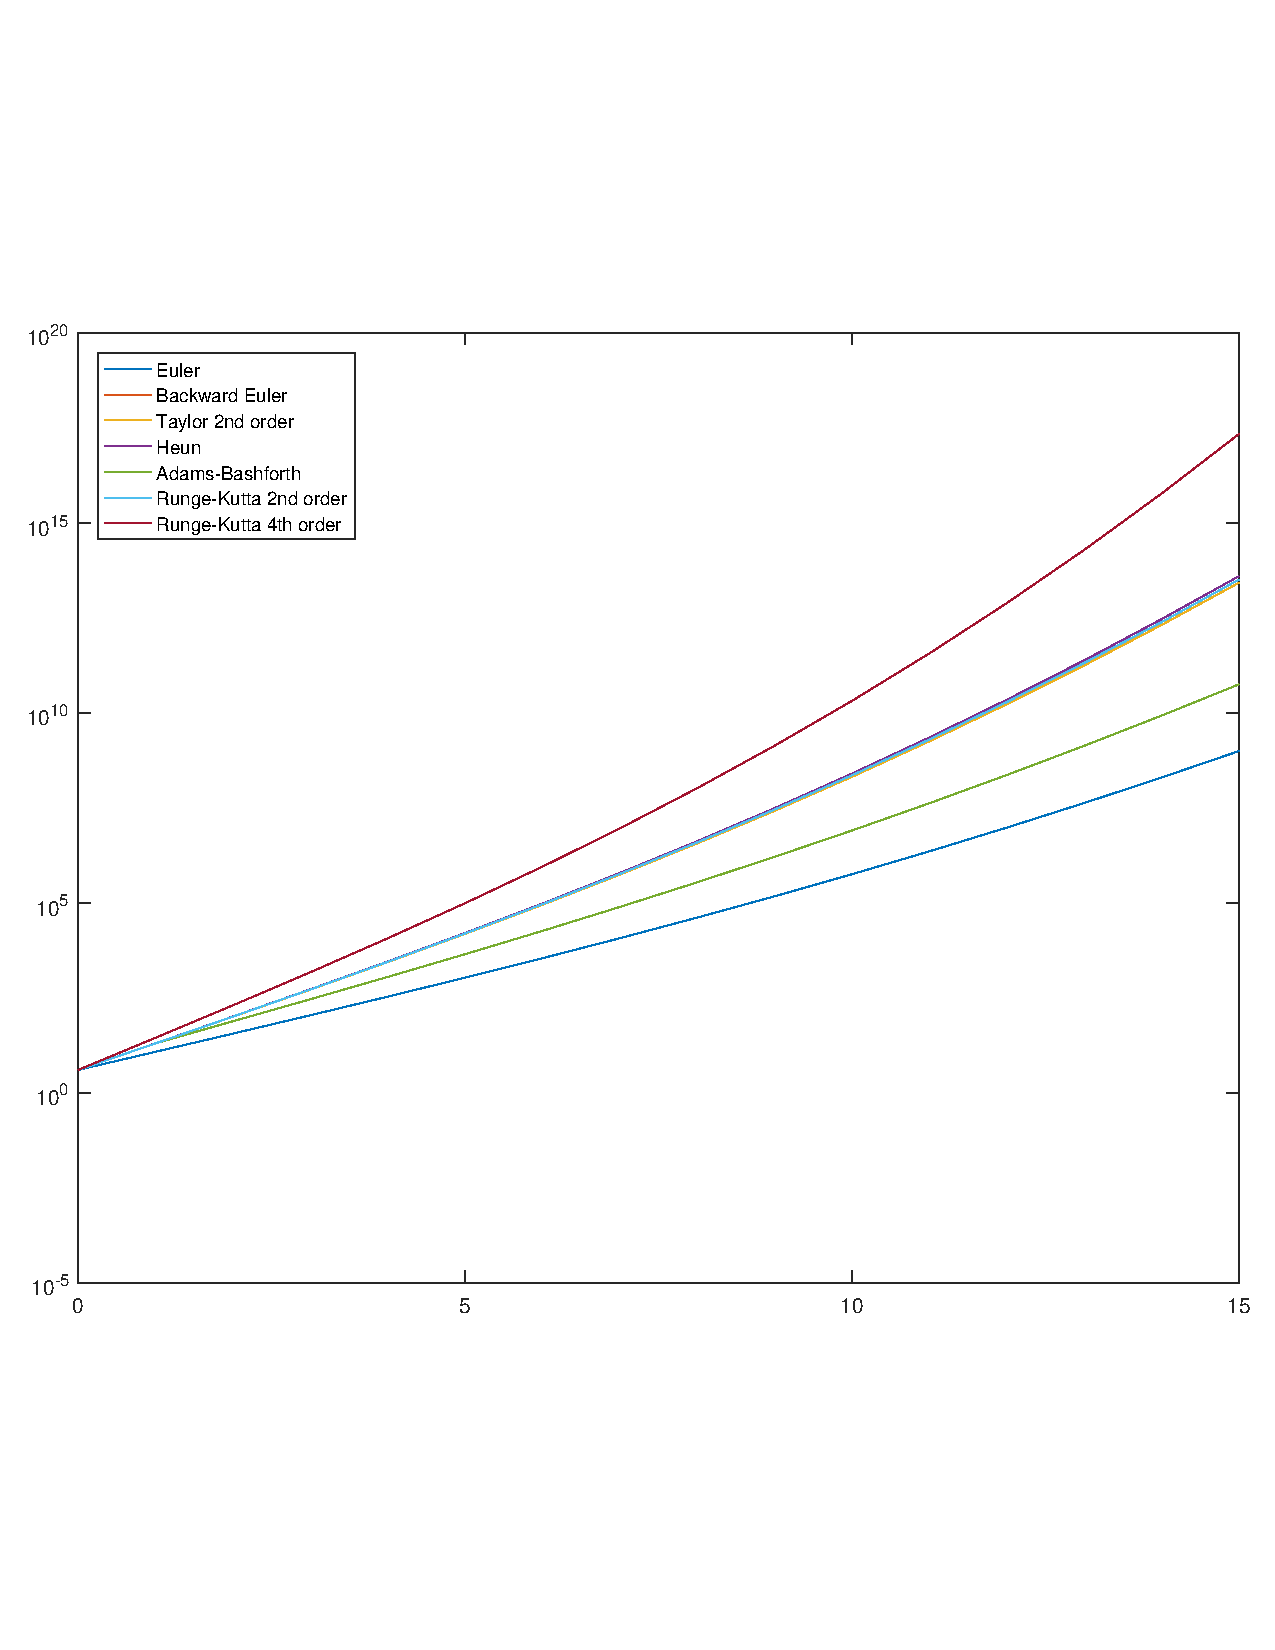
\includegraphics[width=\textwidth]{A9p3.pdf}
	\else
		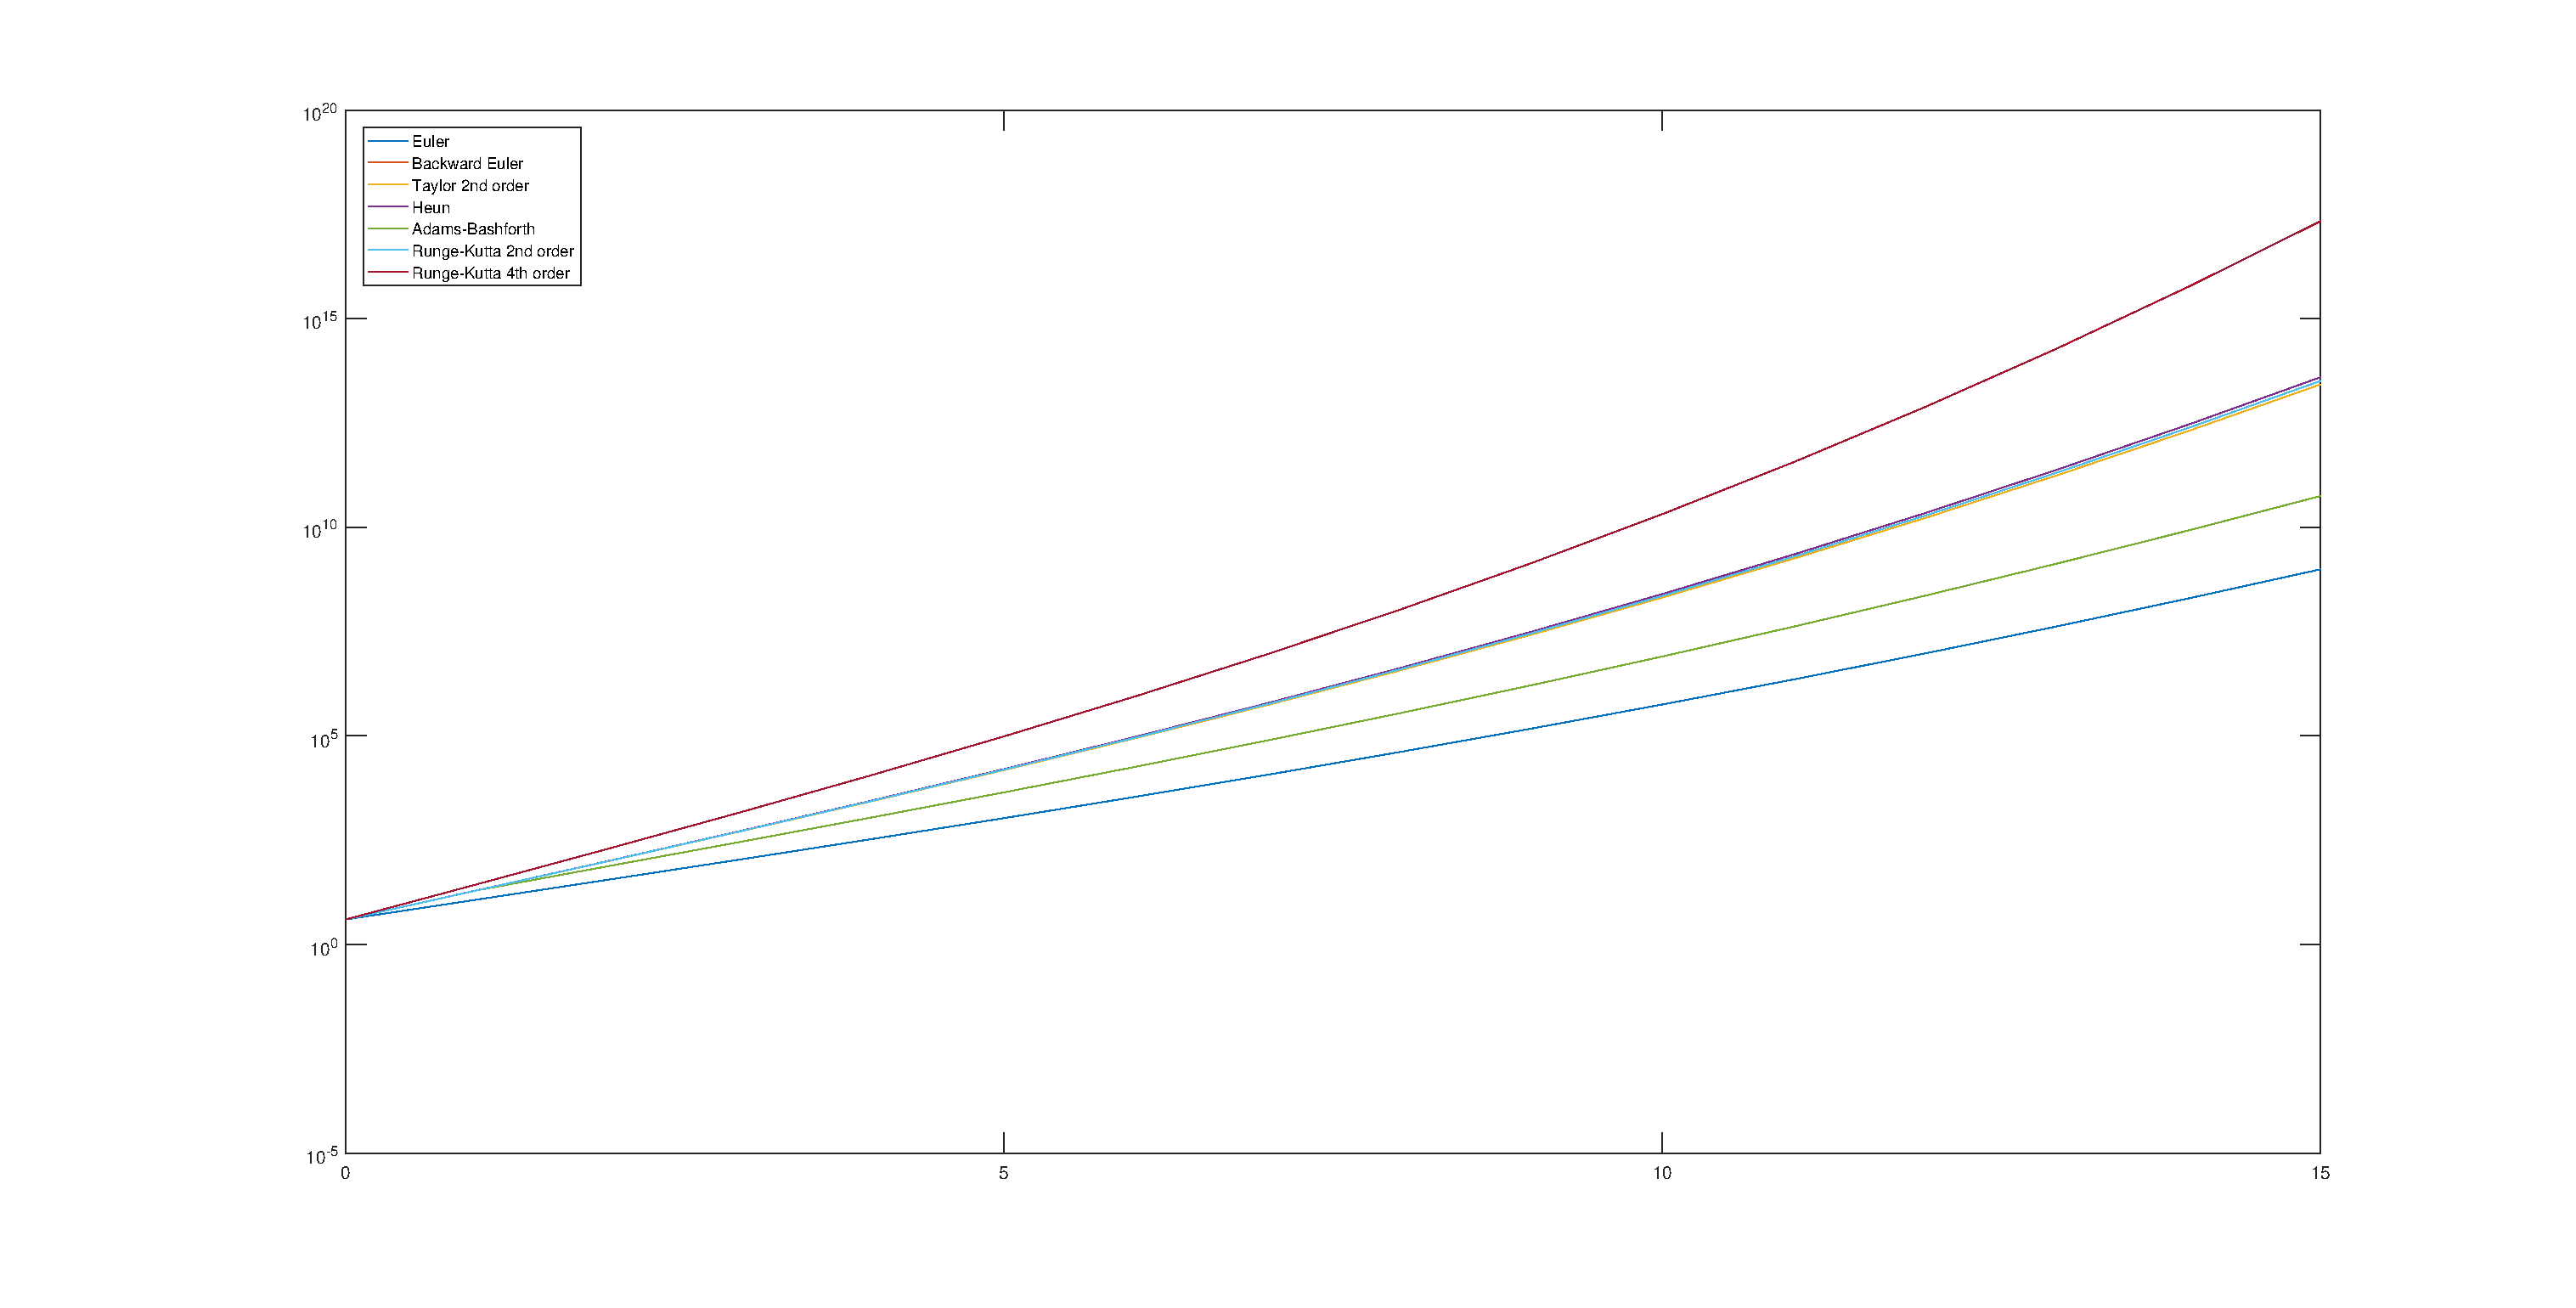
\includegraphics[width=\textwidth]{A9p3.eps}
	\fi
	\caption{Comparison of different methods to solve ODE}
	\label{odecomparisonfig}
\end{figure}


From the figure, we can see that 4\(^\text{th}\) order Runge-Kutta method is the most accurate.
Second-order Taylor's method, Heun's method, two-step Adams-Bashforth method are nearly the same.
Two-step Adams-Bashforth method is worse.
Euler's method is much worse, and backward Euler's method is the worst, since it has negative values and cannot be shown on the graph.



\end{proof}


\section{Classic fourth-order Runge-Kutta method}
Use the classic fourth-order Runge-Kutta method to find the numerical solution of the following higher-order differential equation, and compare the results to the exact solution.
\[ t^3\dddot{y}+t^2\ddot{y}-2t\dot{y}+2y=8t^3-2,\quad y(1)=2, \quad \dot{y}(1)=8, \quad \ddot{y}(1)=6 \]
for \(1\leq t\leq2\) with \(h=0.1\).
The exact solution is
\[ y=-\frac{1}{t}-1+2t+t^2+t^3. \]


\section{Shoot method and Finite-different method}
Solve the following boundary value problem on the domain \(\left[\frac{\pi}{4},\frac{\pi}{3}\right]\) with \(h=\frac{\pi}{60}\)
\[ \ddot{y}=-\left(2\dot{y}^3+\dot{y}y^2\right)\sec t, \quad y\left(\frac{\pi}{4}\right)=\frac{1}{\sqrt[4]{2}}, \quad y\left(\frac{\pi}{3}\right)=\frac{\sqrt[4]{12}}{2}. \]
\begin{enumerate}
	\item By the shoot method.
	\item By the Finite-difference method.
\end{enumerate}


\section{Boundary value problem}
Solve the following BVP on the domain \([0,1]\) by using its variational form
\[ \ddot{y}+\dot{y}+t=0, \quad y(0)=0, \quad y(1)=0. \]
\begin{enumerate}
	\item Assume a linear hat basis for the solution.
	\item Assume a cubic polynomial basis for the solution.
\end{enumerate}


\section{Problem of Runge Kutta method}
Find the following integral using the 4-order Runge Kutta method.
\[ \int_{0}^{1}\left(\frac{1}{(x-0.3)^2+0.01}+\frac{1}{(x-0.9)^2+0.04}-6\right)\ud x. \]
Is equally spaced \(x_k\) the best option for this problem?


\section{Variational form}
Consider the following BVP on the domain \([1,3]\)
\[ x^3y^{(4)}+6x^2y^{(3)}+6xy''-10x=0. \]
The boundary conditions are
\[ y(1)=y(3)=y'(1)=y'(3)=0. \]
\begin{enumerate}
	\item Find its variational form.
	\item Solve it using its variational form.
	\item Compare your solution and the derivative of your solution with the exact solution and its derivative obtained by writing the differential equation as
	\[ \left(x^3 y''\right)''=10x. \]
\end{enumerate}